\documentclass[a4paper]{article}

\usepackage{times}
\usepackage[T1]{fontenc}
\usepackage{a4}
\usepackage{epstopdf}
\usepackage{graphicx}
\usepackage{mathtools}
\usepackage{amssymb}  % lots of math symbols
\usepackage{hyperref}
\usepackage{color}
\usepackage{booktabs}  % nice tables

%% Unicode support
\usepackage[utf8x]{inputenc}
\usepackage{ucs}
\usepackage{autofe}

%% Code
\usepackage{inconsolata}
\usepackage{minted}
\usepackage{fancyvrb}
\usemintedstyle{default}
\newminted{haskell}{gobble=4,linenos,mathescape,fontfamily=tt,fontsize=\footnotesize,xleftmargin=\parindent}




%% Metainformation
%% PDF stuff
\usepackage{datetime}
\usepackage{ifpdf}
\ifpdf
\pdfinfo{
    /Author (Joao Paulo Pizani Flor)
    /Title (A comparison of functional Embedded Domain-Specific Languages for hardware)
    /Keywords (EDSL, HDL, Hardware Description, Functional Programming, Haskell, Coq, Lava, Coquet)
    /CreationDate (D:\pdfdate)
}
\fi

\title{Comparing functional Embedded Domain-Specific Languages for hardware description}

\date{\today}

\author
{
    João Paulo Pizani Flor \\
    Department of Information and Computing Sciences, \\
    Utrecht University - The Netherlands \\
    e-mail: j.p.pizaniflor@students.uu.nl
}



%% The document itself
\begin{document}
    \maketitle

    \section{Introduction}
    \label{sec:intro}
        Hardware design has become nowadays an activity which is, to say the least, extremely
        complex, if not error-prone. The sheer size of circuits has increased. Also, low-level
        concerns such as power consumption, error correction, parallelization and layout
        in general have to be incorporated earlier and earlier in the design process, breaking
        modularity and making it harder to validate and verify the correctness of circuits.

        In this context, researchers have been suggesting for a long time (since the 1980s, in
        fact) the usage of functional programming languages to model circuits. One particular line
        of research is to create Embedded Domain-Specific Languages for hardware description based
        on existing functional programming languages, such as Haskell.

        There is a multitude of EDSLs for hardware description out there, but they vary wildly and
        on a number of aspects: host language, level of abstraction, capabilities of simulation,
        formal verification, synthesis (generation of netlists) and integration with other tools, to
        name a few. All this variety can make the task of choosing a hardware EDSL for the task at
        hand extremely daunting and time-consuming.

        The main goal of this experimentation project is to establish some order in this landscape,
        and to perform a practical analysis of some representative functional hardware EDSLs. By
        reading the materials produced in this project (circuit models, test cases, generated
        netlists, report), a hardware designer wishing to use a functional hardware EDSL for his
        next design should gain some insight about the strengths and weaknesses of each language and
        have an easier time choosing one.

        As an additional result of this research, we intend to identify recent, cutting-edge
        developments in the Haskell language and its implementations that the analyzed EDSLs could
        benefit from. Also, we intend to discuss to which extent some shortcomings of the EDSLs
        could be overcome by having them hosted in a dependently-typed language.

    \section{Methodology}
    \label{sec:methods}
        In this project, we compared a number of functional hardware EDSLs that we considered
        representative (more details on the choice of EDSLs further ahead). The comparison was
        performed on a number of \emph{aspects} for each EDSL, and the analysis was done by
        considering a \emph{sample set of circuits} used as case studies.

        We tried to model all circuits in all EDSLs considered, and as similarly as possible in
        all of them. To avoid using any of the analyzed EDSLs as ``base'', we provide a neutral,
        behavioural description of the circuits.

        \newpage

        \subsection{The languages}
        \label{subsec:languages}
            The embedded Hardware Description Languages we decided to analyze are:
            \begin{description}
                \item[Lava] The Lava\cite{lava1998} language, developed initially at Chalmers
                    University in Sweden.  Lava is deeply embedded in Haskell, and provides features
                    such as netlist generation and circuit verification using SAT-solvers. There are
                    several ``dialects'' of Lava available, and the one used for this project is
                    considered the ``canonical'' one, originally developed at Chalmers.

                \item[ForSyDe] The Haskell ForSyDe library is an EDSL based on the ``Formal System
                    Design'' approach\cite{forsyde1999}, developed at the swedish Royal Institute of
                    Technology (KTH).  It offers both shallow and deep embeddings, and provides a
                    significantly different approach to circuit modelling, using \emph{Template
                        Haskell} to allow the designer to describe combinational functions with
                    Haskell's own constructs.

                \item[Coquet] The Coquet\cite{coquet2011} EDSL differs from the other 2 mainly
                    because it's embedded in a dependently-typed programming language (the Coq theorem
                    prover). Coquet aims to allow the hardware designer to describe his circuits and
                    then \emph{interactively} prove theorems about the behaviour of whole
                    \emph{families} of circuits (using proofs by induction).
            \end{description}

            The Lava EDSL has several ``dialects'', among which are Xilinx-Lava, York-Lava,
            Kansas-Lava and Chalmers-Lava. Xilinx-Lava was developed by Satnam Singh and puts a
            greater emphasis on the \emph{layout} of the described circuits, focusing on their
            implementation in Xilinx's FPGAs. York-Lava was developed as part of the Reduceron
            project, and is a variation of Chalmers-Lava, omitting some features and adding some
            others, like a ``Prelude'' of commonly used circuits ((de)multiplexers, (de)coders,
            etc.), RAM memory blocks, among others. Chalmers-Lava is considered the ``standard''
            dialect, also being the one which was first developed.

            %% TODO
            %% Kansas-Lava

        \subsection{The aspects evaluated}
        \label{subsec:aspects}
            For each of the hardware description EDSLs we experimented with, a number of
            \emph{aspects} were evaluated. The evaluated aspects do not necessarily make sense for
            \emph{all} EDSLs, therefore our presentation follows a language-centric approach, in
            which we expose the strenghts and weaknesses of each EDSL concerning the applicable
            aspects.

            Without further ado, the following aspects are considered in the analysis:

            \begin{description}
                \item[Simulation]
                    The capability of simulating circuits modeled in the EDSL (and the ease with
                    which it can be performed). Simulation is understood in this context as
                    \emph{functional} simulation, i.e, obtaining the outputs calculated by the
                    circuit for certain input combinations.

                \item[Verification]
                    The capability of verifying \emph{formal properties} concerning the behaviour of
                    circuits (and the ease with which verification can be performed). The properties
                    we are interested in are those which are \emph{universally quantified} over the
                    circuit's inputs. As an example of such a property, we might have:
                    \[
                        \forall a \forall b \forall \text{sel}
                            \left( \text{MUX}(a,b,\text{sel}) = a \right)
                            \vee
                            \left( \text{MUX}(a,b,\text{sel}) = b \right)
                    \]

                \item[Genericity]
                    Whether (and how well) the EDSL allows the modelling of \emph{generic} or
                    \emph{parameterized} circuits. An example of a generic circuit is a multiplexer
                    with 2 n-bit inputs and 1 n-bit output, or a multiplexer with n 1-bit inputs and
                    1 1-bit output. Besides parametrization in the \emph{size} if inputs and
                    outputs, we will also analyze whether the EDSL provides chances for
                    parametrization on other functional and/or non-functional attributes.

                \item[Depth of embedding]
                    Whether the EDSL models circuits with a \emph{shallow} embedding (using
                    predicates or functions of the host language), a \emph{deep embedding}
                    (in which circuits are members of a dedicated data type), or anything in
                    between. The depth of embedding of an EDSL might have consequences for other
                    aspects being analyzed.

                \item[Integration with other tools]
                    How well does the EDSL allow for interaction with (getting input from / generating
                    output for) other tools in the hardware design process. For example, synthesis
                    tools for FPGAs or ASICs, timing analysis tools, model checkers, etc.

                \item[Extensibility]
                    The extent to which the user can \emph{add} new interpretations, data types, and
                    combinator forms to the language. For example, the user might want to model
                    circuits that consume and produce custom datatypes, or might be interested in
                    extracting \emph{metrics} from a circuit such as power consumption, number of
                    elementary gates, etc.
            \end{description}


    \section{Modeled circuits}
    \label{sec:circuits}
        When thinking of which circuits to model using the analyzed EDSLs, some principles guided
        us. First of all, they shouldn't be too simple but also not too complex. Some very simple
        circuits (adders, counters, etc.) are very often shown as examples in the papers that define
        the EDSLs themselves, as well as in tutorials. On the other hand, we also did not want to
        model too complex circuits; that would require too much effort on the hardware design
        itself, and diverge from the focus of this project, which is to evaluate and analyze the
        EDSLs.

        Another principle that guided our choice is that the circuits should be immediately familiar
        to anyone with some minimal experience in hardware design. We avoided, therefore,
        considering application-specific circuits such as those for Digital Signal Processing (DSP),
        implementing communication protocols, etc. Having ruled out this class of circuits, we were
        left to choose from circuits that form a general-purpose computing machine, such as
        arithmetic units, memory blocks, control units and so forth.

        Finally, we wanted to choose among circuits that already had a well-defined,
        \emph{behavioural} description, to avoid using any of the analyzed EDSLs as ``basis'' of
        comparison.

        Taking these considerations into account, we chose to implement, in each of the EDSLs
        analyzed, three circuits originating from the book ``The Elements of Computing
        Systems''\cite{nand2tetris-book}. This book aims to give the reader a deep understanding of
        how computer systems work by taking a hands-on approach, in which the reader is given the
        most basic logic gates and builds, step-by-step, all the hardware and software components
        necessary to implement a complete computer system.

        \newpage

        From the hardware design part of the book, we took our three circuits to be modeled:
        \begin{itemize}
            \item A simple Arithmetic Logic Unit (ALU), from here onwards referred to
                as ``circuit 1''.
            \item A RAM memory block with 64 words, from here onwards referred to as ``circuit 2''.
            \item A CPU with an extremely reduced instruction set (capable of executing the
                \emph{Hack} assembly language defined in the book) from here onwards referred to as
                ``circuit 3''.
        \end{itemize}

        \subsection{The ALU circuit}
        \label{subsec:circuit-alu}
            The Arithmetic Logic Unit built by us is a 2-input ALU, in which each of the inputs (as
            well as the output) is a 16-bit long word (interpreted as an integer in two's-complement
            encoding). It is capable of computing several functions, and the choice of which
            function to compute is made by setting the ALU's 6 \emph{control bits}. To become more
            familiar with this circuit, let's first take a look at its block diagram, shown in
            figure \ref{fig:alu-block}
            \begin{figure}[h]
                \begin{center}
                    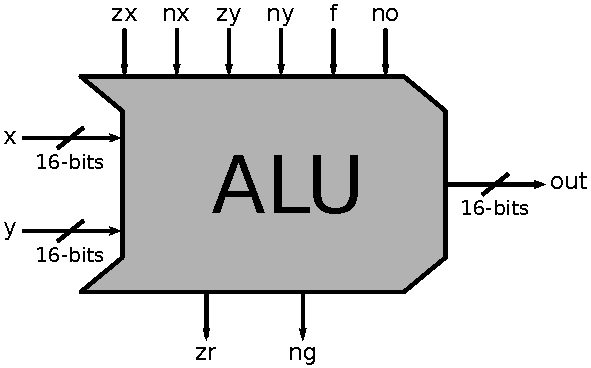
\includegraphics[width=0.6\textwidth]{imgs/alu-block.pdf}
                \end{center}
                \label{fig:alu-block}
                \caption{Block diagram of circuit 1, showing its input and output ports.}
            \end{figure}

            Each of the 6 control bits to the ALU has, in isolation, a well-defined effect on the
            inputs or outputs to the ALU core. The bits \texttt{(zx, nx, zy, ny)} control
            ``pre-processing'' steps for the inputs \texttt{x} and \texttt{y}, with the following
            behaviour:
            \begin{description}
                \item[zx and zy] \emph{Zeroes} the x input (respectively y). The ALU core will
                    receive \texttt{0} as input.
                \item[nx and ny] Performs \emph{bitwise negation} of input x (respectively y).
            \end{description}

            Therefore, the ALU ``core'' itself (adder, and gate) has, as inputs, the results of
            performing these pre-processing steps controlled by \texttt{(zx, nx, zy, ny)}.
            Furthermore, the \emph{output} of the ALU core can also be \emph{bitwise negated} as a
            ``post-processing'' step, controlled by bit \texttt{no}.

            Finally, the control bit $f$ can be used to select which operation is to be performed by
            the ALU core: if we wish to add the two inputs, we need to set $f = 1$, and if we want
            bitwise conjunction, then we need to set $f = 0$.

            Besides the main (16-bit wide) output of the ALU, there are two other output
            \emph{flags}, that indicate predicates over the main output:
            \begin{description}
                \item[zr] Is high whenever $out = 0$.
                \item[ng] Is high whenever $out < 0$.
            \end{description}

            With the ALU in the context of a microprocessor, these flags can be used, for example,
            to facilitate conditional jumps.

            Even though there are $2^{6} = 64$ possible combinations for the values of the control
            bits, only 18 of these combinations result in interesting functions -- that because
            several combinations of control bits can be used to calculate the same function. We show
            these 18 functions that the ALU can calculate on table \ref{tab:alu-functions}.
            \begin{table}[h]
    \begin{center}
        \begin{tabular}{ccccccc}
            \toprule
            \textbf{zx} & \textbf{nx} & \textbf{zy} &
            \textbf{ny} & \textbf{f} & \textbf{no} & \textbf{out=}
            \tabularnewline
            \midrule

            1  &  0  &  1  &  0  &  1  &  0  &   $0$  \\

            1  &  1  &  1  &  1  &  1  &  1  &   $1$  \\

            1  &  1  &  1  &  0  &  1  &  1  &   $-1$  \\

            0  &  0  &  1  &  1  &  0  &  0  &   $x$  \\

            1  &  1  &  0  &  0  &  0  &  0  &   $y$  \\

            0  &  0  &  1  &  1  &  0  &  1  &   $\neg x$  \\

            1  &  1  &  0  &  0  &  0  &  1  &   $\neg y$  \\

            0  &  0  &  1  &  1  &  1  &  1  &   $-x$  \\

            1  &  1  &  0  &  0  &  1  &  1  &   $-y$  \\

            0  &  1  &  1  &  1  &  1  &  1  &   $x + 1$  \\

            1  &  1  &  0  &  1  &  1  &  1  &   $y + 1$  \\

            0  &  0  &  1  &  1  &  1  &  0  &   $x - 1$  \\

            1  &  1  &  0  &  0  &  1  &  0  &   $y - 1$  \\

            0  &  0  &  0  &  0  &  1  &  0  &   $x + y$  \\

            0  &  1  &  0  &  0  &  1  &  1  &   $x - y$  \\

            0  &  0  &  0  &  1  &  1  &  1  &   $y - x$  \\

            0  &  0  &  0  &  0  &  0  &  0  &   $x \wedge y$  \\

            0  &  1  &  0  &  1  &  0  &  1  &   $x \vee y$  \\

            \bottomrule
        \end{tabular}
    \end{center}
    \label{tab:alu-functions}
    \caption{Functions that the ALU can calculate, given different settings of the control bits}
\end{table}


            %% Talk about the construction of the ALU in terms of its parts.


        \subsection{The RAM circuit}
        \label{subsec:ram-circuit}
            Circuit 2 is a block of RAM with 64 lines and in which each line is a 16-bit word.
            Actually, using the term ``RAM'' to refer to this component is an abuse of terminology,
            as this circuit is nothing more than a register bank.

            All the input and output ports of the circuit are pictured in its block diagram, shown
            in figure \ref{fig:ram-block}.
            \begin{figure}[h]
                \begin{center}
                    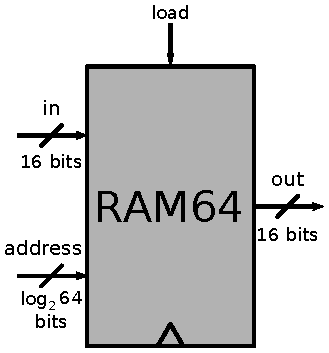
\includegraphics[width=0.4\textwidth]{imgs/ram-block.pdf}
                \end{center}
                \label{fig:ram-block}
                \caption{Block diagram of circuit 2, a RAM of 64 lines}
            \end{figure}

            The circuit has one 16-bit output, named ``out'', and three inputs (``in'', ``address''
            and ``load''). The ``in'' port is 16-bit wide and holds a value to be written into the
            RAM. The ``address'' port has a width of $\log_{2} 64 = 6$ bits and holds the address
            in which reading or writing is to be performed. Finally, the 1-bit ``load'' input
            controls whether the value currently at ``in'' should be written to the selected
            address. There is also one \emph{implicit} input for a clock signal in this component.
            Implicit, in this case, means that the clock signal is not present in any of the models
            that we developed for this circuit, but must be present at any physical implementation.

            The temporal behaviour of this memory block is as follows: At any point in time, the
            output ``out'' holds the value stored at the memory location specified by ``address''.
            If the ``load'' pin is high, then the value at ``in'' is loaded into the memory word
            specificied by ``address''. The loaded value will then be emitted on the output at the
            \textbf{next} clock cycle.

        \subsection{The Hack CPU circuit}
        \label{subsec:hack-cpu-circuit}
            Circuit 3, the largest and most complex circuit among the ones we have chosen to
            implement, is the Central Processing Unit for the \emph{Hack} computer, the machine
            described in the book ``The Elements of Computing Systems''\cite{nand2tetris-book}.

            The Hack computer is based on the \emph{Harvard architecture}, that means that it has
            different storage component and signal pathways for instructions and data. Therefore,
            the Hack CPU expects to be connected to \emph{two} memory blocks, the instruction memory
            and the data memory. Having this in mind facilitates the understanding of the CPU's
            block diagram, shown in figure \ref{fig:cpu-block}
            \begin{figure}[h]
                \begin{center}
                    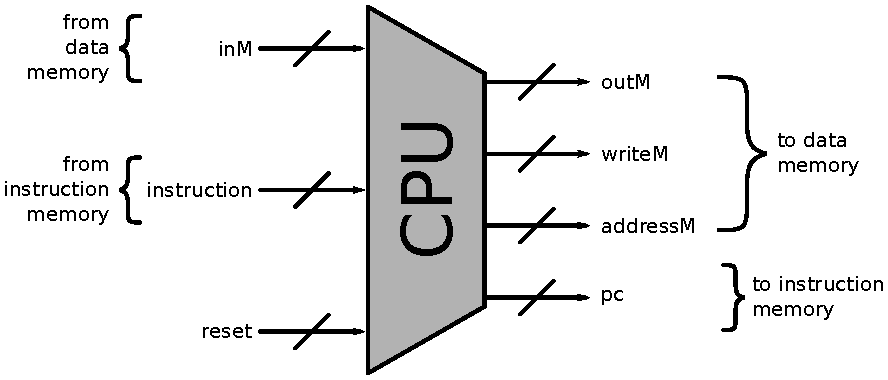
\includegraphics[width=0.9\textwidth]{imgs/cpu-block.pdf}
                \end{center}
                \label{fig:cpu-block}
                \caption{Block diagram of circuit 3, the Hack CPU}
            \end{figure}

            The Hack architecture has an \emph{extremely} reduced instruction set, and consists in
            fact of only two instructions (each 16-bit wide): A (meaning ``address'') and
            C (meaning ''compute''). The A instruction can be used as a means to load numerical
            literals into the data memory, as well as setting a special ``cache'' register inside
            the CPU. The C instruction is the one responsible for effectively performing
            computations using the ALU, testing outputs and jumping. More details about programming
            in the Hack assembly language can be found in \cite{nand2tetris-book}.

            The meaning of each of the CPU's input and output ports becomes much clearer when we
            look at the context in which the CPU is inserted, namely, the memory modules to which it
            is connected. So, let's analyze the CPU's ports by taking a look at figure
            \ref{fig:cpu-memory}.
            \begin{figure}[h]
                \begin{center}
                    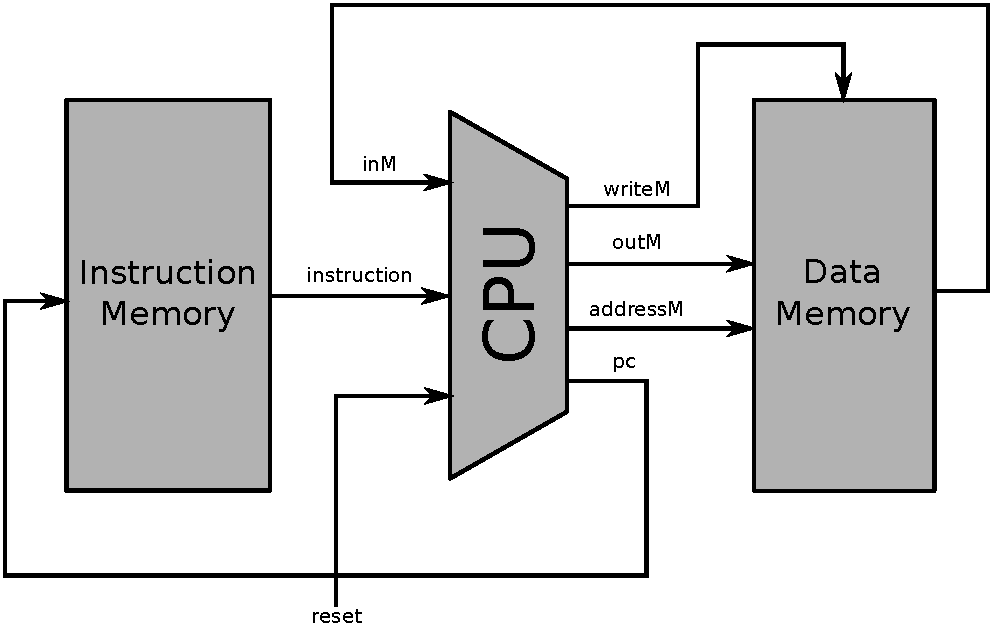
\includegraphics[width=1.0\textwidth]{imgs/cpu-memory.pdf}
                \end{center}
                \label{fig:cpu-memory}
                \caption{The Hack CPU connected to the data and instruction memory blocks}
            \end{figure}

    \section{Analysis of the EDSLs}
    \label{sec:edsls}

        \subsection{Lava}
        \label{subsec:lava}
            The Lava EDSL\ldots

        \subsection{ForSyDe}
        \label{subsec:forsyde}
            The Haskell ForSyDe library is an implementation of the ``Formal System Design''
            approach to hardware modelling\cite{forsyde1999}. The ForSyDe approach per se has
            several significant differences when compared to Lava, and even when the two EDSLs agree
            on \emph{what to do}, sometimes they differ on how to achieve those goals.

            To better understand what characterizes the ForSyDe methodology, we first have to
            establish some vocabulary:
            \begin{description}
                \item[System] In ForSyDe, a system or circuit is a network of processes
                    interconnected by \emph{signals}.
                \item[Signal] A signal is, intuitively, a stream of information that flows between
                    processes. More concretely, it carries events of some type, and each event has
                    an associated tag. The meaning of the tag is defined by the \emph{model of
                    computation}\ref{subsubsec:forsyde-mocs} used.
                \item[Process] A process is nothing more than a pure function on signals. A process
                    \emph{is able} to hold internal state. But, given the same input (possibly
                    infinite) signals, it produces the same output signals.
                \item[Process constructor] Every ciruit in ForSyDe, even simple combinational ones,
                    is built with a \emph{process constructor}. A process constructor can be seen as
                    a skeleton of behaviour, and it clearly separates computation from
                    synchronization aspects. A process constructor takes a combinational function
                    (called \emph{process function}) as parameter -- expressing the computation
                    aspect of the process, and possibly some extra values. There are combinational
                    and sequential process constructors, and some representative examples from each
                    class will be described in more detail in a specific subsection
                    \ref{subsubsec:forsyde-synchprocs}.
            \end{description}

            % Talk about models of computation
            \subsubsection{Models of Computation}
            \label{subsubsec:forsyde-mocs}
                The definition of signal given above is purposefully ``vague'' mainly because the
                precise definition of signals is given by the \emph{model of computation} being
                used. ForSyDe has (currently) process constructors for the following models of
                computation:
                \begin{description}
                    \item[Synchronous] Lorem ipsum  %% TODO
                    \item[Untimed] Lorem ipsum
                    \item[Continuous] Lorem ipsum
                \end{description}

                Among those, perhaps the most ``notable'' one is the Synchronous MoC, because it
                reflects the usual interpretation of signals as wires and the vast majority of
                digital designs nowadays having a global clock. Also, all of our studied circuits
                were modelled in ForSyDe using the Synchronous MoC. Therefore, it is interesting to
                take a deeper look at it.

                First, lets take a look at the behaviour of a system which has an one integer input
                port and one integer output, and in which the value of the output is equal to the
                input plus 4. The interface and internal architecture of this system
                (\emph{addFour}) is depicted in figure \ref{fig:forsyde-addFour}.
                \begin{figure}[h]
                    \begin{center}
                        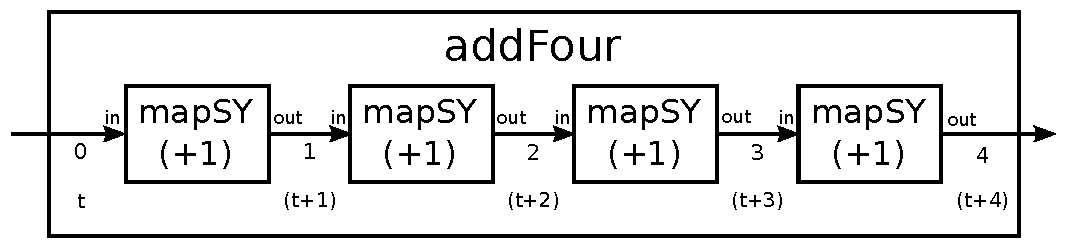
\includegraphics[width=1.0\textwidth]{imgs/forsyde-addFour.pdf}
                    \end{center}
                    \label{fig:forsyde-addFour}
                    \caption{The addFour circuit, example of usage of the Synchronous MoC}
                \end{figure}

                In this system, each of the constituent processes is built using the \texttt{mapSY}
                process constructor, a constructor of the synchronous model of computation (its name
                ends in ``SY''). It takes a combinational function (in this case ``+1'') and
                evaluates it for each event in the input signal, generating a corresponding event in
                the output signal.

            \subsubsection{Synchronous Process Constructors}
            \label{subsubsec:forsyde-synchprocs}

            %% TODO
            % Talk about shallow and deep embedded signals (deep only supports synchronous)
            % Disadvantages: name handling, not actively maintained
            % Advantages: more modular VHDL generated (hierarchical). Higher-level descriptions

        \subsection{Coquet}
        \label{subsec:coquet}
            The third analyzed EDSL for hardware description, Coquet\cite{coquet2011},
            is strikingly different from both others. Most of these differences can be explained in
            one way or another by its choice of host ``language'' -- Coq.\footnote{``Coq'' is not
                the name of a language, but a theorem-proving system that uses different languages
                for defining terms, interactive commands, and user-defined tactics}

            Coq is an interactive theorem prover based on \emph{intuitionistic type theory}. In the
            context of Coq, the concepts of ``term'' and ``type'' are far more intertwined than,
            say, in Haskell. Types in Coq can contain references to terms and vice-versa. A very
            typical example of these so-called \emph{dependent types} is the type(-family) of
            vectors with a certain length:
            \begin{verbatim}
    Inductive vec A : nat -> Type :=
        | nil  : vec A 0
        | cons : forall (h : A) (n : nat),  vec A n -> vec A (S n).
            \end{verbatim}

            By having the length of the vector being part of the type, we can \emph{enforce} several
            useful properties of functions operating on vectors. In fact, the type-system of Coq is
            so expressive that it can encode any proposition of \emph{intuitionistic propositional
                logic}, a formal logic in which almost all of mathematics can be proven.

            Given such expressive power, one can imagine that it might be useful to express circuits
            in Coq, and use it to prove interesting properties about these circuits. This is exactly
            the goal of Coquet. How this goal is achieved and the modelling of our studied circuits
            in Coquet is discussed in the following subsections.

            \subsubsection{Modelling circuits}
            \label{subsubsec:coquet-modelling}
                Coquet is a deep-embedded DSL, thus it represents circuits as a datatype. By using
                dependent types, a designer modelling a circuit in Coquet is able to prevent certain
                kinds of ``errors'' much earlier in the design process, because the
                \emph{well-formedness} is guaranteed by construction, i.e, every circuit built using
                the constructors provided by Coquet are well-formed by definition. Let's take a look
                at the \emph{Circuit} data type definition:
                \begin{verbatim}
    Context {tech : Techno}
    Inductive ℂ : Type -> Type -> Type :=
    | Atom : ∀ {n m : Type} {Hfn : Fin n} {Hfm : Fin m}, techno n m -> ℂ n m
    | Plug : ∀ {n m : Type} {Hfn : Fin n} {Hfm : Fin m} (f : m -> n), ℂ n m
    | Ser : ∀ {n m p : Type}, ℂ n m -> ℂ m p -> ℂ n p
    | Par : ∀ {n m p q : Type}, ℂ n p -> ℂ m q -> ℂ (n + m) (p + q)
    | Loop : ∀ {n m p : Type}, ℂ (n + p) (n + p) -> ℂ n m
                \end{verbatim}

                The \texttt{ℂ} type is parameterized by two types (in the definition above
                represented by the letters n, m, p\ldots). These types are the \emph{input} and
                \emph{output} types of the circuit, respectively. These parameters can be
                instantiated to any types which have instances for the \texttt{Fin} type class.
                These types \textbf{do not} represent what is ``carried'' on the wires, on the other
                hand, they are meant to represent the ``structure'' of the input and output ports:
                basically how many of them there are, how are they grouped and how are they named.

                %% Parameterized by techno, the fundamental gate of the technology

                %% Example sum circuit
                %% Tags for facilitating distinction

                % Example of circuit: Adder

            \subsubsection{Circuit semantics in Coquet}
            \label{subsub:coquet-semantics}



            % Improvements:
            % * Coquet has already meaning relations defined in the context of streams. A stream is
            %   a function from nat -> A. With we generalize on the nat, we can approximate
            %   ForSyDe's concept of Signal.


    \section{Results summary}
    \label{sec:results}

    \section{Conclusions}
    \label{sec:conclusions}


    \bibliographystyle{plain}
    \bibliography{references}


%% Expected outputs of this project
%% ================================
%% The main output I expect from this project is a comparative analysis of the EHDLs. An interesting
%% side-product will be the code describing the case study circuits in the various languages. This
%% code shall hopefully be useful as a learning source for people interested in experimenting with
%% functional hardware design.
%% 
%% Last, but not least, one output of this project which I also find interesting is the set of
%% comparison criteria itself, along with the justification of why they were chosen.


\end{document}
